\documentclass[times, 10pt,twocolumn]{article}

\usepackage{sose2011}
\usepackage{times}
\usepackage{color}
\usepackage[pdftex]{graphicx}

\graphicspath{{./images/}}
\DeclareGraphicsExtensions{.pdf,.jpeg,.png,.jpg}

% correct bad hyphenation here
\hyphenation{op-tical net-works semi-conduc-tor}
\pagestyle{empty}

\begin{document}

\title{Managed Control of Composite Cloud Systems}

\author{
        \textbf{Christopher Lamb}\hspace*{0.3in}
        \textbf{Pramod Jamkhedkar}\hspace*{0.3in}
        \textbf{Greg Heileman}\hspace*{0.3in}
        \textbf{Chaouki Abdullah}\\
        Department of Electrical and Computer Engineering \\
        University of New Mexico \\
        \small{\{cclamb, pramod54, heileman, chaouki\}@ece.unm.edu}
}

\maketitle
\thispagestyle{empty}

\begin{abstract}
Cloud providers have just begun to provide primitive functionality enabling users to configure and easily provision resources, and primarily in the Infrastructure as a service domain at that.  In order to effectively manage cloud resources in an automated fashion, systems must automate quality of service metric measurement as a part of a larger usage management strategy.  Collected metrics can then be used within control loops to manage and provision cloud resources when needed.  This basic approach can be scaled to monitor the use of system artifacts as well as simple quality-of-service parameters, and can also address the needs of large systems spanning the boundaries of single service providers.
\end{abstract}

{
\setlength{\parindent}{0mm}
\textbf{Keywords:} Usage Management, Cloud Computing, System of Systems.
}

\section{Introduction}
Cloud computing services as a computational paradigm are more market oriented than previous attempts at commodity computing.  Furthermore, they are in many cases designed to be composed into larger, more powerful customer facing systems.  These kinds of aggregate systems fit neatly into one of the more commonly used definitions of a system of systems as well \cite{Sose:SageCuppan:2001}, \cite{Sose:Web:Defns}.  With so much data in the hands of different providers in an aggregate system, system developers and users are hard-pressed to effectively monitor and control the use of sensitive content by various composite systems.  Some of this information can be contained in Service Level Agreements (SLAs), but they have thus far been focused on quality-of-service (QoS) metrics rather than addressing issues like data flow or physical application residency.  For the most part SLAs are simply not sufficient for addressing usage management concerns \cite{WSA}, \cite{WSLA}, \cite{WSP}, \cite{PaRaSh:09}.

Effective usage management monitoring coupled with feedback processing creates an event loop suitable for applying control theoretic concepts to cloud infrastructures.

Usage policies specified at a fine-grained level provides cloud service users with more reliability of the use of their data within cloud centric systems.  For example, data routing, caching, or hosting can be a sensitive issue for some systems in that specific users may want to restrict the countries that can access that data.  The ability to specify and control where specifically that data travels and resides gives those kinds of sensitive users confidence to use could-centric computing resources.  Furthermore, this kind of control will also facilitate cost profiles for services that more closely match demand, giving providers better control over their infrastructure and additional areas for product differentiation.

Herein, we will elaborate the idea of applying usage management to single and distributed could systems.  In this brief analysis, we will touch on the application of common system design principles and standards \cite{BlCl:01}, \cite{Cl:88}, \cite{ClWrSoBr:02}, application of usage control concepts \cite{PaSa:04}, \cite{JaHeLa:10}, policy language application \cite{JaHeMa:06}, digital rights management (DRM) systems~\cite{JaHe:09}, and interoperability~\cite{JaHe:04}, \cite{HeJa:05}, \cite{KoLaMaMi:04}, \cite{coral}, \cite{marlin}.  We will apply these ideas toward a controllable feedback-enabled system suitable for cloud system control.

In Section~\ref{sec:single} this paper first addresses how to create a controllable system with feedback suitable for system evaluation from the perspective of a single provider. Here, we will address the constraints and advantages of such an approach and how providers could begin to offer these kinds of services.  In this first example, we will focus on QoS data specifically.  Next in Section~\ref{sec:singleUm} we will extend our single provider system to provide control over attributes more specific to the usage management domain, with examples and associated analysis.  Finally in Section~\ref{sec:multiple} we extend this single provider model to a more realistic system deployed to multiple cloud providers in a realistic system-of-systems scenario.

\subsection{Previous Work}
Could computing is emerging as the future of utility systems hosting for consumer-facing systems.  In these kinds of systems, components, applications, and hardware are provided as utilities over the Internet with associated pricing schemes pegged by system demand.  Users accept specific QoS guidelines that providers use to provision and eventually allocate resources. These guidelines become the basis over which providers charge for services.

Over the past few years multiple service-based paradigms like web-services, cluster computing and grid computing have contributed to the development of what we now call cloud computing~\cite{Bu:09}. Cloud computing distictly differentiates itself from other service-based computing paradigms by via a collective set of distinguishing characteristics:  market orientation, visualization, dynamic provisioning of resources, and service composition via multiple service providers~\cite{BuYeVeBrBr:09}. This implies that in cloud computing, a cloud-service consumer's data and applications reside inside that cloud provider's infrastructure for a finite amount of time  Partitions of this data can in fact be handled by multiple cloud services, and these partitions may be stored, processed and routed through geographically distributed cloud infrastructures. These activities occur within a cloud, giving the cloud consumer an impression of a single virtual system.  These operational characteristics of cloud computing can raise concerns regarding the manner in which of cloud consumer's data and applications are managed within a given cloud. Unlike other computing paradigms with a specific computing task focus, cloud systems enable cloud consumers to host entire applications on the cloud (i.e. Software as a Service). As consumers aggressively start exploiting these advantages to transition IT services to external utility computing systems, the manner in which data and applications are handled within those systems by various cloud services will become a matter of serious concern.   

%The handling or use of consumer data within the cloud by different services refers to the policies regarding constraints under which different actions may be carried out on the data. A cloud consumer might want to limit the way in which data is stored, routed, or processed, and specify who is authorized to carry out these activities and under what conditions. As an example, a government agency might want to prevent the data from being stored in one particular country, or prevent the routing of its data via a particular set of networks it considers unreliable. Similarly, a financial company might want to prevent its data from being processed by a particular cloud service, or may want it to be encrypted before being stored by an untrusted cloud storage service. Usage policies typically consists of a range of semantics such as restrictions on the manner in which data is used, temporal restrictions on usage, spacial or attribute-based restrictions, permissions, obligations, penalties, count-based limits on usage and partial dependencies to name a few.   Hence, as cloud services become pervasive, cloud consumers will want to dictate the terms of usage for their data and applications within the cloud in a manner that is expressive enough to capture the concerns of cloud users. At present, cloud providers enable these features via rudimentary techniques by offering a one-size-fits-all options to consumers. For example, Amazon S3 storage services allow a region-based facility where data stored in one region is guaranteed not to leave that particular region~\cite{AWS}. Future cloud computing services will need to enable these terms to be expressed in SLAs in a sophisticated, fine-grained manner that will allow the cloud consumers to express the usage terms explicitly. 

%As mentioned earlier, service expectations in service-based computing paradigms are expressed in terms of SLAs negotiated with the service provider. For different types of service-based computing paradigms such as web services, clusters, and grid computing, there exist well established SLA frameworks that enable expression, interpretation, monitoring, control and enforcement of SLA terms~\cite{WSA, WSLA, WSP,PaRaSh:09}. However, the SLAs supported by these frameworks focus on performance metrics such as availability, reliability, bandwidth, response times, instructions per second, etc. ~\cite{PaSc:06}. Also, the privacy and security metrics supported by these frameworks focus primarily on encryption of the data. It must be noted that usage policies are significantly different than these metrics and present a new dimension that is orthogonal to the manner in which the other metrics are managed. It is therefore necessary to have a separate mechanism for usage management in cloud computing environments. The next section discusses the characteristic features of such a framework.


%\begin{figure}[!t]
%\centering
%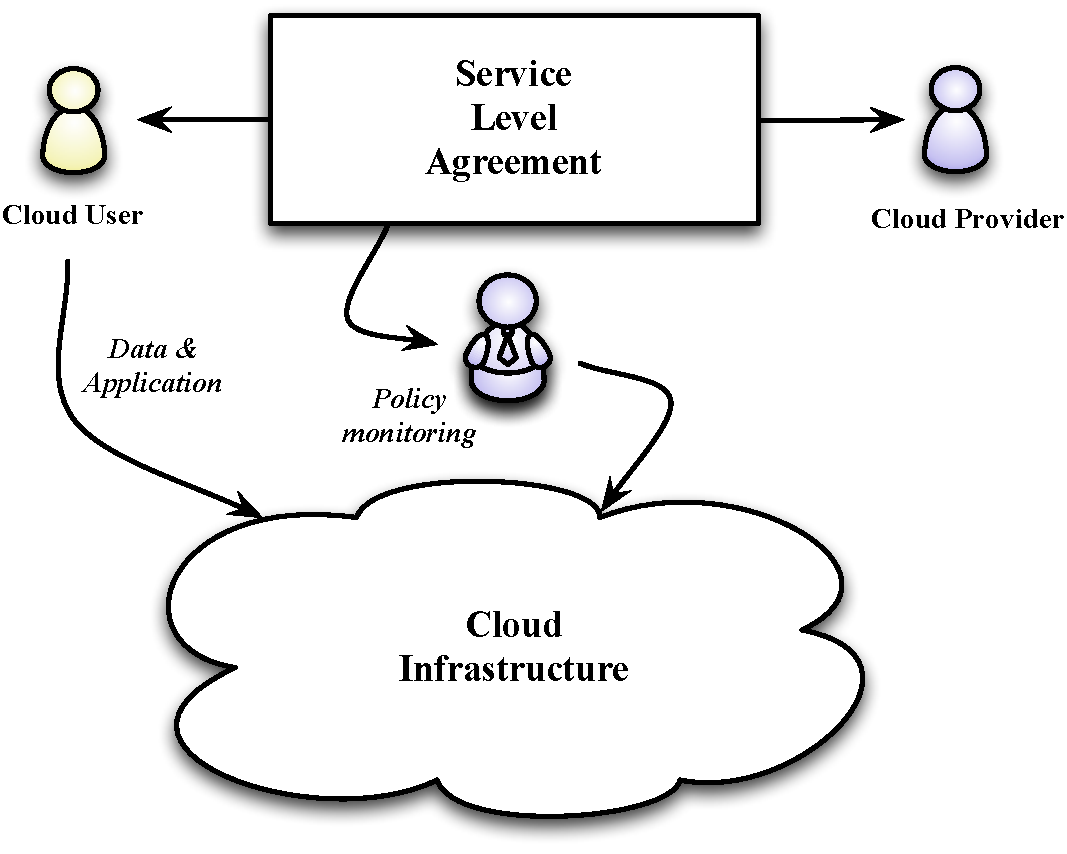
\includegraphics[width=3in]{Overview.pdf}
%\caption{Overview of the manner in which SLAs are implemented in present cloud environments.}
%\label{fig:overview}
%\end{figure}

%\cite{Emr:Web:Jade,Emr:Web:Fipa}.
%\cite{KoLaMaMi:04,SaShUe:04}

\section{Single Provider Feedback System}\label{sec:single}
Controllable cloud systems enable providers to supply more closely targeted, cost effective services while at the same time providing service consumers with the confidence that the data and other artifacts their systems use are protected.  With that as our eventual goal, we first begin with a simple system managing currently accepted QoS parameters - system attributes like bandwidth, system memory allocation, and the like.  Specifically, we intend to provide the ability to monitor and control a virtual system hosted on a cloud infrastructure so that response time for a hosted application falls within a specific range of accepted parameters.

In order to manipulate a system to meet a preselected threshold of performance metrics, we must have access to measurement information with respect to factors effecting those metrics and we need to be able to adjust system performance in response to those measurements.  We are going to focus on system response time measured at the edge of the cloud provider's infrastructure as the metric we wish to control.  We are going to adjust system performance to meet that metric by manipulating the number of processing nodes, bandwidth available to those nodes, and node RAM allocations.

We have identified the attributes we wish to control.  This leads us to a group of requirements we can use to assemble a logical system architecture.  Requirements we know we need to address include:

\begin{itemize}
\item \textit{Performance:} We will be adjusting a system within specific soft real-time frames.  Ergo, we need to be able to collect feedback measurements, process those measurements, and make decisions about how to respond to those measurements quickly in order to avoid falling out of compliance with any performance parameters to which we must adhere.
\item \textit{Accessibility:} In order to control component systems, we must be able to access those systems.  In order to do so within time constraints, we must be able to access those systems electronically as well; physical access requirements simply will not scale into this performance domain.
\item \textit{Controllability:} We must be able to access the appropriate control primitives on the systems we need to tune.  This will include accessing compute node generation and termination capabilities.  It would help if we could access node performance information and tune those nodes as well, though this is not required; we can emulate this by terminating nodes in one configuration and creating nodes with another to more adequately address performance needs.
\end{itemize}

These system attributes lead us to a system architecture that is beginning to look like a traditional feedback-centric controllable system.
\\
\\
\textcolor{red}{[insert UML diagram]}
\\
\\
The above system has four primary components, one of which has three subcomponents.  These components work together to provide cloud services to consumers in a hypothetical Infrastructure-as-a-Service scenario.  This particular view addresses logical, functional components of this kind of a system rather than specific technologies used in an implementation, although some components are loosely modeled on popular open-source cloud environments (i.e. Eucalyptus).

Essentially, we have a cloud controller element that initiates provisioning of compute nodes within a given cluster. The cluster itself is managed by a cluster controller, which in turn controls storage controllers, node controllers, and by extension, nodes.  The nodes and node controllers themselves are monitored by a resource allocation controller which refers to a set of QoS requirements.

\begin{itemize}
\item \textit{Cloud Controller:} Provides an initial interface to administrative users to control the cloud.
\item \textit{Cluster Controller:} Managed by the cloud controller, the cluster controller manages the resources of a single cluster. A given cloud may contain multiple clusters.
\item \textit{Storage Controller:} Provides storage of system images and for other general storage needs.  This controller component is highly I/O sensitive.
\item \textit{Node Controller:} Responsible for allocating, delivering, and managing individual compute nodes upon which client software runs.  This is the primary computational resource accessed by users accessing managed cloud resources.
\item \textit{Node:} The compute node delivering services to end users and managed by the cluster's control infrastructure.
\item \textit{QoS:} Quality of service terms the cloud provider has agreed to honor for the cloud customer with respect to system delivery, provisioning, and overall performance.
\item \textit{Resource Allocation Controller:} The component responsible for real-time tuning of the cloud system to maintain defined quality of service.
\end{itemize}

Operationally, the initial commands required to initialize the cloud are delivered from the \textit{Could Controller} to the \textit{Cluster Controller}, who then propagates another, related set of commands provisioning an initial set of resources from the \textit{Node Controllers} and the \textit{Storage Controllers}.  At this point, the initial system has been configured and is running, serving hosted software to it's customer base.

Once the system is running, state data describing the performance metrics of interest is dispatched from \textit{Nodes} on the \textit{Node Controllers} and the \textit{Storage Controller} and delivered to the \textit{Resource Allocation Controller}.  The \textit{Resource Allocation Controller} then processes this new event data in the context of the defined \textit{QoS} parameters.  This processing, in this model, is likely to be simple processing over the current event package or perhaps the current and the otherwise most recent event package.  This evaluation is very performance sensitive; we need to process the state of the current system quickly and adjust resource allocation accordingly.  Because of this soft real-time requirement, we do not have the luxury of spending significant time reviewing trending or providing sophisticated analysis over delivered event information.  Note that extension of this system into the feedforward domain would allow this kind of more robust system management, allowing us to employ more complex and powerful machine learning or neural systems to predict system needs.

Finally, if needed the \textit{Resource Allocation Controller} will dispatch messages to the \textit{Cluster Controller}, \textit{Nodes}, and \textit{Storage Controller} adjusting system profiles to ensure they remain within acceptable performance ranges.
\\
\\
\textcolor{red}{[cast in control theoretic terms, include block diagram]}
\\
\\
This control infrastructure as it has strict timing requirements with respect to event collection, analysis, and control, likely needs to be hosted in close physical proximity to the controlled systems.  Otherwise, the systems themselves can be located just about anywhere accessible to the Internet.  These logical components are not necessarily all hosted on physically distinct systems either, though generally at least the \textit{Storage Controller} and the \textit{Node Controller} are as they have remarkably different requirements with respect to processing power and I/O throughput.

Clearly, both the cloud service consumer and providers are impacted by this kind of infrastructure.  Consumers have systems performing within required performance bounds, and providers are no longer required to maintain as strict administrative over-watch of managed systems.  This kinds of systems may also impact system developers, as this kind of dynamic node control and allocation imparts new requirements with respect to intra-system data handing and processing.  Generally however, accepted service development guidelines with respect to statelessness and allowing running processes to terminate prior to node shutdown will alleviate these issues.

When implemented, this kind of system will provide dynamic runtime control of cloud systems enhancing provider and customer confidence in the hosted infrastructure's performance potential.  This can also be extended into the usage management realm with more specific requirements with respect to how customer artifacts are managed, not just delivered.

\section{Single Provider Feedback System with Usage Management}\label{sec:singleUm}
Now that we have developed a cloud system capable of fairly granular control via a feedback control 
loop using QoS parameters, we will being to incorporate specific usage management parameters.  
Usage management, as a field, extends simple access control and digital rights management 
perspectives with regard to resources.  While access control is concerned with controlling access to a 
specific protected resource, usage management incorporates control over that initial access and 
extends into how that resource is used after that initial access.  Likewise, while digital rights 
management technologies do exert some level of control over the use of artifacts, they have generally 
been applied in strict media domains like music, film, or digitized images.  In this system we will 
apply usage management to specific non-traditional artifacts to control how they are used and where 
they may be stored.  

In order to provide control over customer data artifacts in a cloud environment, we need to first 
establish a basic mechanism for doing so.  This system must fit within the functional confines of the 
QoS system from Section \ref{sec:single} while extending the QoS functionality to artifacts not generally 
controlled via traditional QoS metrics.  For these purposes, a good example of an artifact not 
generally controlled via QoS parameters could be streaming network data.  While bandwidth 
throttling is clearly in the QoS domain, more specific uses of that data stream like caching and 
routing are not.  

Using a data stream as an example, we recognize some situations we clearly need to be able to 
control.  In this example, we will limit ourselves to a data stream emitted from a \textit{Node} on a 
\textit{Node Controller} which is routed to a user as a result of a user request.  Here, we have control 
over stream creation.  We want to limit the ability to update that data stream, we certainly don't want 
that stream deleted, and we want to limit who may read that stream.  In fact, we can safely assume in 
this scenario that update and deletion are operations we want to completely forbid, while we may 
want to limit stream readability, leading us to the primary new requirement when adding usage 
management over a network stream in this case:

\begin{itemize}
\item \textit{Accessibility:} Data streamed through the cloud system must be able to be monitored and the 
accessibility of that stream needs to be dynamically tunable.  This implies that we need to be able to 
control routing and caching of all streaming data according to user specified conditions.  This also 
implies that we need to be able to control exactly which \textit{Node Controllers} are able to spawn 
which \textit{Nodes}.
\end{itemize}

The addition of these attributes and requirements give us this logical system:
\\
\\
\textcolor{red}{[insert UML diagram w/ UM \& network components]}
\\
\\
(what; present UML diagram of single system with QoS)
[insert UML diagram, with new elements]
	(describe how they work together)
	(cast in control theoretic terms)
(where; discuss where it would be hosted)
	(address physical and logical)
(how; discuss how this supports better management of cloud systems)
(who; who is impacted and how they're impacted)

\textcolor{red}{[expand to UM, add new components and implications]}

\section{Scaling to Multiple Providers}\label{sec:multiple}

\textcolor{red}{[scale to multiple providers accessing common QoS]}

\section{Conclusion}
In this paper we introduced the notion of usage management in cloud computing environment. Cloud computing exhibits a unique set of characteristics that will require usage management of users' data according to user concerns and expectations. We analyzed the challenges involved in the design and development of a framework for usage management in cloud environments. We showed that such a framework needs to be open to leverage existing security technologies and SLA frameworks. The framework needs to exhibit features such as support for multiple policy languages, existence of a common cloud ontology, dynamic interpretation and data transformations. Finally a preliminary framework that supports multiple policy languages was introduced that will provide a platform upon which such a framework can be built. 

Future works involves efforts towards the development of a common extensible cloud ontology that will provide the vocabulary underlying this framework and enable interoperability. Such an ontology needs be developed by taking into consideration the requirements of different cloud services. In addition, it is necessary to standardize interfaces for other security mechanisms mentioned in the paper that can be incorporated within the framework. Finally, the framework allows use of multiple policy languages, to this effect, existing policy languages can be modified to be incorporated within the framework, and news ones need to designed to address the specific needs of different cloud services.



\bibliographystyle{IEEEtran}
\bibliography{emr,drm,sose}

\end{document}


